\documentclass[12pt]{article}

\usepackage{amsmath}
\usepackage{hyperref}
\usepackage{graphicx}

\begin{document}

\begin{titlepage}
    \centering
    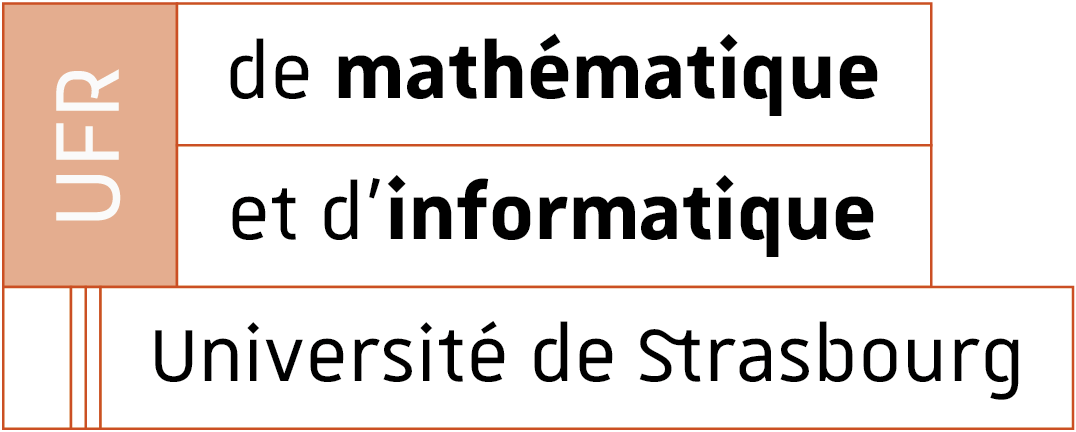
\includegraphics[width=0.5\textwidth]{images/logo_ufr.png}\par\vspace{1cm}
    \vspace{1.5cm}
    {\huge\bfseries ExaMA WP1 - Vegetation\par}
    \vspace{2cm}
    {\Large Giulio Carpi Lapi, Pierre-Antoine Senger\par}
    \vfill
    supervised by\par
    Pierre Alliez and Vincent Chabannes

    \vfill

% Bottom of the page
    {\large Date: \today\par}
\end{titlepage}

\tableofcontents
\newpage

\section{Abstract}
We are given a 3D geometric model of an urban area (neighborhood, city, etc.),
including the geometry of the buildings and the terrain.
This allows us to create a numerical model for thermal and energy simulation.
The purpose of this project is to integrate the vegetation into the model,
since the vegetation, particularly trees,
can have a significant influence on the model.
To do that we are going to follow the following steps:

\begin{itemize}
    \item Access the OpenStreetMap database to retrieve the position of trees
    (and other information such as size if available).
    \item Generate a library of 3D tree models.
    \item Integrate these models into a terrain mesh.
\end{itemize}

V1:

\begin{itemize}
    \item Methodology
    \item Results
    \item Conclusion
\end{itemize}

\section{Introduction}
Urban areas are complex environments where various factors interact to influence 
microclimates, energy consumption, and overall livability. Among these factors, 
vegetation, particularly trees, plays a crucial role in shaping the urban landscape 
and its environmental characteristics. Trees provide shade, mitigate heat, reduce 
air pollution, and enhance the aesthetic appeal of neighborhoods and cities. Their 
strategic placement and characteristics can significantly impact the thermal and 
energy dynamics of urban areas.

In recent years, advancements in computational modeling have facilitated the 
development of sophisticated tools for simulating the thermal and energy performance 
of urban environments. These tools rely on 3D geometric models that accurately 
represent the built environment, including buildings, roads, and terrain. However, 
the integration of vegetation into these models remains a challenge, despite its 
recognized importance.

The integration of vegetation into 3D urban models poses several challenges. 
Obtaining accurate data on the location, size, and species of trees within an 
urban area is non-trivial. Additionally, representing the complex geometry of trees 
in a scalable and computationally efficient manner is a significant computational 
challenge. Nevertheless, addressing these challenges is essential for creating 
realistic and reliable simulations that account for the influence of vegetation on 
urban microclimates and energy usage.

In this context, this project aims to develop a methodology for integrating 
vegetation, particularly trees, into 3D geometric models of urban areas. Leveraging 
data from sources such as the OpenStreetMap database, the project seeks to identify 
the position and attributes of trees within the urban landscape. Subsequently, a 
library of 3D tree models will be generated to accurately represent the vegetation 
in the model. Finally, these tree models will be integrated into the terrain mesh, 
enabling comprehensive simulations that consider the interactions between buildings, 
terrain, and vegetation.

By incorporating vegetation into 3D urban models, this project seeks to enhance the 
accuracy and realism of thermal and energy simulations. The resulting models will 
provide urban planners, architects, and policymakers with valuable insights into 
the environmental performance of urban areas, ultimately contributing to the 
development of more sustainable and resilient cities.


\section{Literature Review}

\section{Methodology}

\section{Results}

\section{Conclusion}

\section{References}
\nocite{*}
\bibliographystyle{plain}
\bibliography{references}

\end{document}